\section{Applying EarlyDiscard and JITL to Wearable Cognitive Assistants}
\label{bw:wca}

While the experiments in previous sections
(~\ref{sec:earlydiscard}~\ref{sec:jitl}) are performed in a drone video
analytics context, EarlyDiscard and JITL approaches can be applied more
generally to live video analytics offloading from Tier-3 devices to Tier-2 edge
data-centers. In this section, we use the LEGO
application~\cite{chen2018application} to showcase how to apply these bandwidth
saving approaches to WCAs.

\begin{figure}
    \centering
    \begin{minipage}[]{0.45\linewidth}
        \centering
        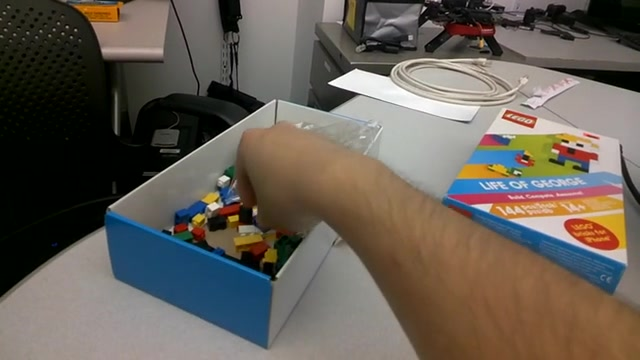
\includegraphics[width=\linewidth]{FIGS/lego-search}\\
        {(a) Searching for Lego Blocks}
    \end{minipage}
    \begin{minipage}[]{0.45\linewidth}
        \centering
        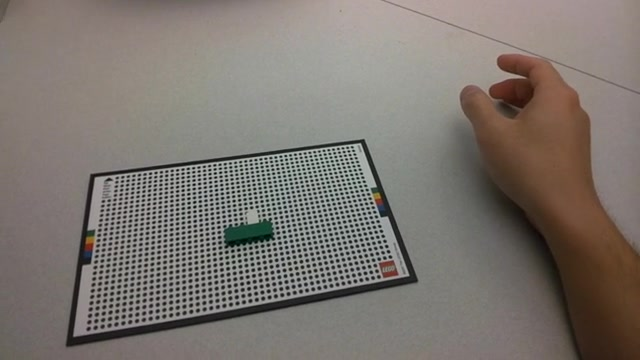
\includegraphics[width=\linewidth]{FIGS/lego-assembled}\\
        {(b) Assembling Lego Pieces}
    \end{minipage}
    \caption{Example Images from a Lego Assembly Video}
    \label{fig:wca-lego-example-images}
\end{figure}

The LEGO wearable cognitive assistant helps a user put together a specific Lego
pattern by providing step-by-step audiovisual instructions. The application
works as follows. The assistant first prompts a user an animated image showing
the Lego block to use and asks the user to put it on the Lego board or assemble
it with previous pieces. Following the guidance, the user searches for the
particular Lego block, assemble it, and put the assembled piece on the Lego
board for the next instruction. Figure~\ref{fig:wca-lego-example-images} shows
the first-person view images captured from the wearable device during this
process. The assistant analyzes the assembled Lego piece on the Lego board by
identifying its shape and color using computer vision and provides the suitable
instruction.

\begin{figure}
    \centering
    \begin{minipage}[]{0.31\linewidth}
        \centering
        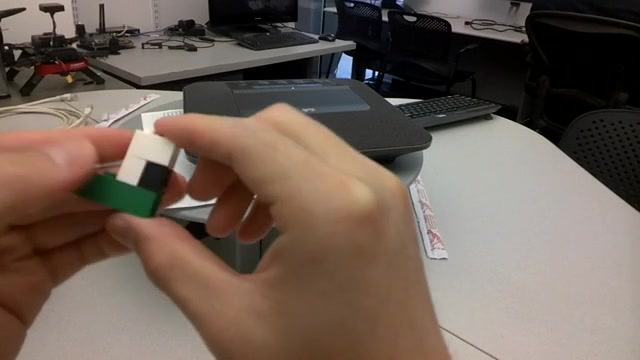
\includegraphics[width=\linewidth]{FIGS/lego-dataset-1}\\
    \end{minipage}
    \begin{minipage}[]{0.31\linewidth}
        \centering
        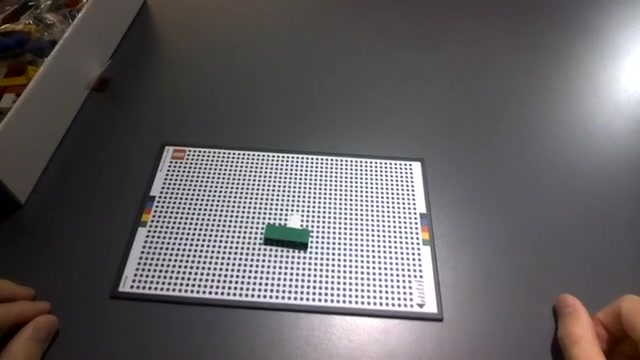
\includegraphics[width=\linewidth]{FIGS/lego-dataset-2}\\
    \end{minipage}
    \begin{minipage}[]{0.31\linewidth}
        \centering
        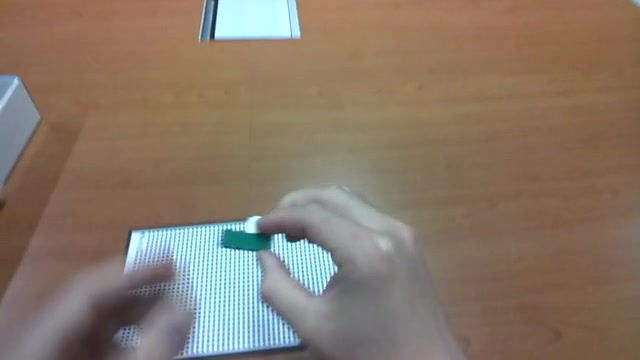
\includegraphics[width=\linewidth]{FIGS/lego-dataset-3}\\
    \end{minipage}
    \caption{Example Images from LEGO Dataset}
    \label{fig:wca-lego-dataset}
\end{figure}

Intuitively, to the assistant, frames capturing the assembled piece on the Lego
board, (for example Figure~\ref{fig:wca-lego-example-images} (b)) are the
crucial frames to process, as they reflect the user's working progress.
Figure~\ref{fig:wca-lego-example-images} (a), on the other hand, is less
interesting as it does not contain information on user progress. If some cheap
processing on the wearable device could distinguish
(a) from (b), bandwidth consumption can be
reduced as we can discard Figure~\ref{fig:wca-lego-example-images} (a) early on
the wearable device without transmitting the frame to the cloudlet for processing.
This provides opportunities to apply EarlyDiscard and JITL.

We collect a LEGO dataset of twelve videos, in which users assemble Lego pieces
in three environments with different background, lighting, and viewpoints.
Figure~\ref{fig:wca-lego-dataset} shows example images from the dataset. We run
the LEGO WCA on these videos to get pseudo ground truth labels. Specifically,
for each frame, based on the outputs of the LEGO WCA vision processing, we
categorize the frame to be either ``interesting'' or ``not interesting''. A
frame is considered to be interesting if a LEGO board is found in the frame,
otherwise considered not interesting.

\begin{figure}
    \centering
    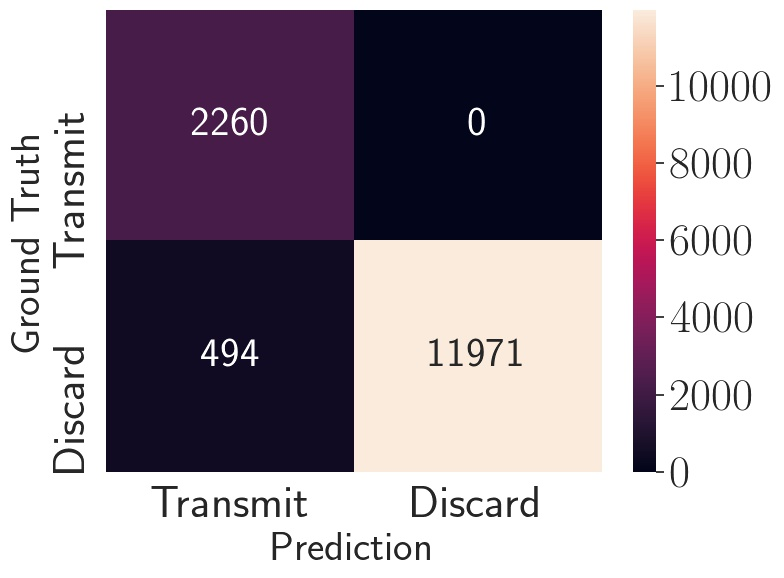
\includegraphics[width=.6\linewidth]{FIGS/earlydiscard-cm}\\
    \caption{EarlyDiscard Filter Confusion Matrix}
    \label{fig:wca-early-discard}
\end{figure}

We use this dataset to finetune a MobileNet DNN in order to automatically
distinguish interesting frames from the boring ones for EarlyDiscard. For each
of the three environments, we randomly select two videos for training, one video
for validation, and one video for testing. We randomly sample 2000 interesting
images and 2000 boring images from the six training videos as the training
data. Similarly, we random sample 200 interesting images and 200 boring images
from the three validation videos as the validation data. We implement
MobileNet transfer learning using the PyTorch
framework~\cite{paszke2019pytorch}. We train the model for 20 epochs and
select the model weights that give the highest accuracy on the validation set as
the model for inference.

Our test sets have in total 14725 frames. Figure~\ref{fig:wca-early-discard}
shows the confusion matrix of our trained EarlyDiscard classifier. X-axis
represents the predicted results: ``Transmit'' means the frame is predicted to
be interesting and should be transmitted to cloudlet for processing while
``Discard'' means the frame is predicted to be boring and should not be
transmitted. Similarly, Y-axis represents the ground truth results. As we can
see, the classifier correctly predicts 2260 out of 14725 frames to be
interesting and correctly suppresses 11971 frames. With EarlyDiscard in place,
only 19\% of all the frames are transmitted. Meanwhile, the false negative is 0
frame, meaning no ``interesting'' frame is wrongly discarded. This is the result
of biasing the classifier towards recall instead of precision.

\begin{figure}
    \centering
    \begin{minipage}[b]{.45\linewidth}
        \centering
        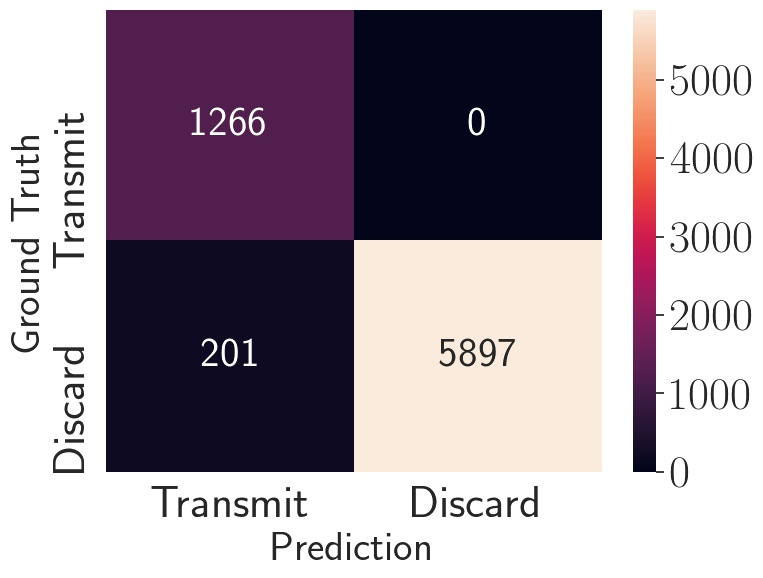
\includegraphics[width=\linewidth]{FIGS/jitl-earlydiscard-cm}\\
        {(a) EarlyDiscard}
    \end{minipage}
    \begin{minipage}[b]{.45\linewidth}
        \centering
        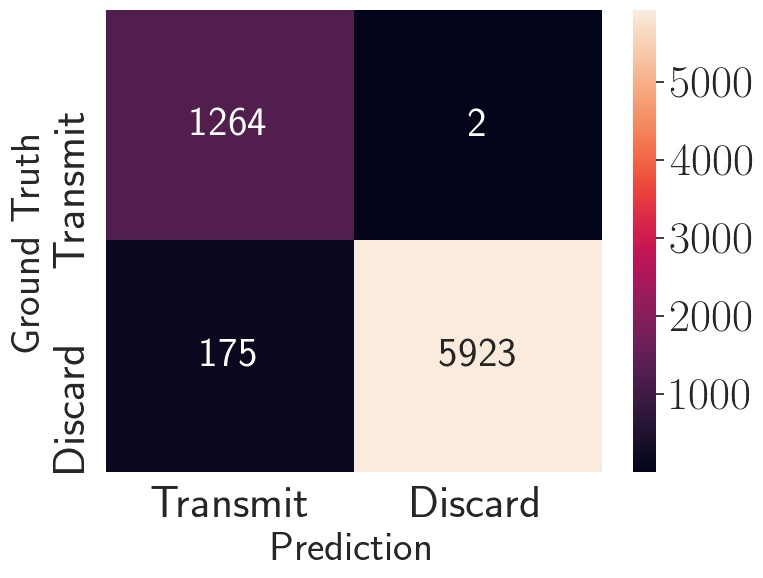
\includegraphics[width=\linewidth]{FIGS/jitl-combined-cm}\\
        {(b) EarlyDiscard + JITL}
    \end{minipage}
    \caption{JITL Confusion Matrix}
    \label{fig:wca-jitl}
\end{figure}

Among all the frames that are transmitted, 18\% of them are false positives.
These 494 false positives suggest that there are room to improve using JITL. For
each of the test videos, we use the first half of the video as training examples
for JITL to train a SVM that produces a confidence score for EarlyDiscard
prediction. Figure~\ref{fig:wca-jitl} compares the confusion matrix of using
EarlyDiscard alone with EarlyDiscard + JITL. As we can see, JITL reduces 13\% of
the false positives at the cost of 2 false negatives. Note that these 2 false
negative frames do not result in missing instructions as adjacent interesting
frames are still transmitted.

% To reduce bandwidth consumption with EarlyDiscard and JITL, we first need to
% identify what frames should be considered interesting.

% the cheap computer vision processing that can identify ``interesting'' frames on
% Tier-3 devices. Figure~\ref{fig:wca-lego-example-images} provides intuitions on how to
% apply EarlyDiscard and JITL to the Lego application